% Chapter 1
\chapter{مقدمه}

\section{شناخت موضوع}
در سال‌های اخیر، به دلیل پیشرفت‌های سریع فناوری و دسترسی آسان به اینترنت، بسیاری از دستگاه‌ها به اینترنت متصل شده‌اند. این پدیده که به اینترنت اشیا%
\LTRfootnote{Internet of Things}
معروف است، شامل انواع دستگاه‌ها از جمله دستگاه‌های پوشیدنی%
\LTRfootnote{Wearable Devices}%
، خودروهای خودران، خانه‌های هوشمند%
\LTRfootnote{Smart Homes}
و به ویژه تلفن‌های هوشمند%
\LTRfootnote{Smart Phones}
می‌شود. این دستگاه‌ها به طور چشمگیری زندگی روزمره انسان‌ها را دگرگون کرده‌اند. استفاده از این سیستم‌ها همگی باعث تولید حجم قابل توجهی داده در طول روز می‌شوند که شرکت‌های بزرگ فناوری از این داده‌ها بهره برده و با استفاده از آن‌ها اقدام به ارائه انواع سرویس به کاربران خود می‌نمایند.

با پیشرفت علم هوش مصنوعی و استفاده گسترده از روش‌های یادگیری ماشین، امکان بهره‌برداری بهینه از حجم عظیم داده‌های تولید شده فراهم گردیده است. این داده‌ها می‌توانند برای اجرای الگوریتم‌های مختلف به منظور دستیابی به اهداف متنوع به کار گرفته شوند. روش‌های متعددی برای مدیریت و اجرای این الگوریتم‌های یادگیری وجود دارد که در ادامه به توضیح هر یک پرداخته خواهد شد.


\subsection{یادگیری متمرکز}
روش یادگیری متمرکز%
\LTRfootnote{Centralized Learning}
که در بسیاری از سیستم‌های امروزی به کار می‌رود، به این صورت عمل می‌کند که تمامی گره‌ها%
\LTRfootnote{Nodes}
اطلاعات خود را به صورت کامل به سرویس‌دهنده ابری%
\LTRfootnote{Cloud Server}
ارسال می‌کنند. سرویس‌دهنده ابری با دسترسی به تمامی داده‌ها، الگوریتم‌های مورد نظر را اجرا می‌کند
\cite{elbir2022family}.
این روش در شکل
\ref{centralized_learning}
به تصویر کشیده شده است.


\subsection{یادگیری غیر متمرکز}
در روش یادگیری غیر متمرکز%
\LTRfootnote{Decentralized Learning}
، هر گره به صورت مستقل الگوریتم‌های مورد نظر را اجرا می‌کند. پس از چند مرحله اجرای کد، اطلاعات به‌روز شده را با گره‌های همسایه به اشتراک می‌گذارد. این فرآیند تا زمانی ادامه می‌یابد که تمامی گره‌ها به یک مقدار مشخص همگرا شوند
\cite{zhou2019edge}.
این روش در شکل
\ref{decentralized_learning}
به نمایش در آمده است.


\subsection{یادگیری توزیع شده}
در روش یادگیری توزیع‌شده%
\LTRfootnote{Distributed Learning}
، یک هسته مرکزی مسئولیت مدیریت کل سیستم و تمامی داده‌ها را بر عهده دارد. با این حال، به دلیل نیاز به توان پردازشی بالا، این هسته بار پردازشی را بین گره‌های موجود تقسیم می‌کند. این تقسیم بار باعث می‌شود که فرآیند آموزش سریع‌تر و کارآمدتر انجام شود. همچنین، امکان استفاده همزمان از منابع مختلف برای تحلیل داده‌های بزرگ، فراهم می‌شود.
این روش در شکل
\ref{distributed_learning}
نشان داده شده است.


\begin{figure}[b]
	\centering
	\subfigure[
	یادگیری متمرکز
	\cite{zhou2019edge}.
	]{
		\label{centralized_learning}
		\includegraphics*[width=.31\textwidth]{images/chap1/centralized_learning.png}
	}
	\hspace{0.5mm}
	\subfigure[
	یادگیری غیرمتمرکز
	\cite{zhou2019edge}.
	]{
		\label{decentralized_learning}
		\includegraphics*[width=.31\textwidth]{images/chap1/decentralized_learning.png}
	}
	\hspace{0.5mm}
	\subfigure[یادگیری توزیع‌شده.]{
		\label{distributed_learning}
		\includegraphics*[width=.31\textwidth]{images/chap1/distributed_learning.png}
	}
	\caption{انواع روش‌های یادگیری}
	\label{learning_methods}
\end{figure}



\section{یادگیری فدرال}
سیستم‌های متمرکز تا پیش از این بیشتر نیازها را برطرف می‌کردند، اما در دنیای امروزی و با افزایش تعداد دستگاه‌های متصل، چالش‌های جدیدی مطرح شده است. هزینه‌های بالای ناشی از انتقال حجم زیاد داده‌ها از یک جهت، و افزایش نگرانی‌ها درباره امنیت اطلاعات حساس و شخصی از جهت دیگر، محققان را به سمت استفاده از الگوریتم‌های غیرمتمرکز و توزیع‌شده در حوزه یادگیری ماشین سوق داده است. یکی از جدیدترین زیرمجموعه‌های مهم و پرکاربرد روش‌های یادگیری توزیع‌شده، یادگیری فدرال است که بسیار مورد توجه قرار گرفته است.


در روش یادگیری فدرال، برخلاف رویکردهای متمرکز یادگیری ماشین، تجزیه و تحلیل داده‌ها به دستگاه‌های لبه%
\LTRfootnote{Edge Devices}
یا کاربران%
\LTRfootnote{Clients}
منتقل می‌شوند
\cite{ma2022state}.
این روش، به عنوان یک جایگزین مطلوب برای مدل‌سازی داده‌ها در محیط‌هایی با تعداد زیادی کاربر معرفی شده است. در این چارچوب، به جای انتقال داده‌های اصلی، پارامترهای مدل‌های محلی در هر مرحله از فرآیند آموزش به سمت سرور منتقل می‌شوند، که این امر توانایی بهبود امنیت و کاهش هزینه‌های ارتباطی را فراهم می‌کند.
در شکل
\ref{federated_learning}
این معماری به نمایش گذاشته شده است.


 \begin{figure}[t]
	\centering
	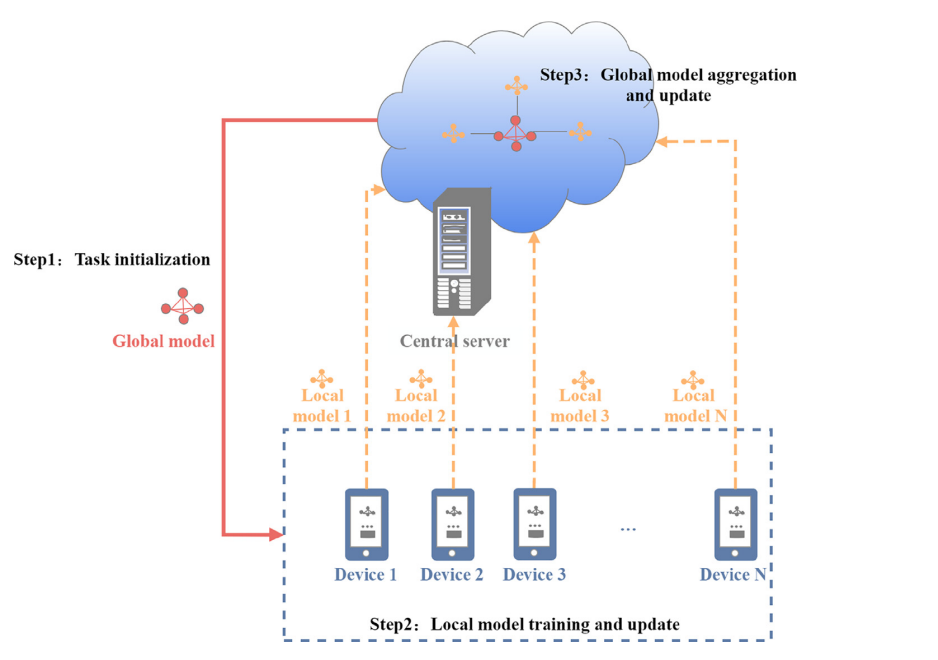
\includegraphics[scale=0.7]{images/chap1/federated_learning.png}%
	\caption{%
		یادگیری فدرال 
		\cite{ma2022state}%
		.
	}
	\label{federated_learning}
	\centering
\end{figure}

سرور در حقیقت نقش رهبری را ایفا می‌کند و با توجه به نوع داده‌ها، یک مدل شبکه عصبی%
\LTRfootnote{Neural Network}
ایجاد کرده و آن را به سمت کاربران ارسال می‌کند. در ادامه کاربران با توجه به داده‌های خود شبکه را آموزش می‌دهند و بعد از چند بار تکرار به صورت محلی، وزن‌های به‌روزرسانی شده را به سمت سرور بر می‌گردانند. همان‌طور که در شکل
\ref{federated_learning}
مشاهده می‌شود، داده‌ها همگی در سمت کاربران قرار گرفته‌اند و به سمت سرور ارسال نمی‌شوند. عدم اجبار در به اشتراک گذاشتن اطلاعات گره‌ها در یادگیری فدرال، کمک شایانی به حفظ حریم شخصی کاربران می‌کند
\cite{smith2017federated}.





% ابتدای فصل بهار سال 2017 محققین گوگل (Google) طی یک مطلب کوتاه در وبلاگ هوش مصنوعی، برای اولین بار موضـوع یادگیری فدرال را تحـت مطلبی با عنوان "یادگیری فدرال: یادگیری ماشین اشتـراکی، بدون آموزش متمرکز داده‌ها" مطرح نمودند. در این مطلب به طور کوتاه Google Keyboard یا به اختصار Gboard معرفی شد که با به کاری‌گیری یادگیری فدرال، لغت بعدی را پیش‌بینی و به کاربر توصیه می‌نمود. یادگیری فدرال در این کاربرد، نیاز به ارسال داده‌های کاربران به سمت سرور را حذف کرده است و به طور محلی مدل را به‌روزرسانی می‌کند.
%بنابراین، با بهره‌گیری از اطلاعات پنهان بسیار زیاد دستگاه‌ها در فرآیند مدل‌سازی، ضمن حفظ حریم شخصی سرویس‌گیرنده‌ها خدمات بهتری نسبت به قبل ارائه می‌گردد. در شکل نحوه استفاده از یادگیری فدرال در این برنامه به نمایش درآمده است.



\section{تاریخچه یادگیری فدرال}


در اوایل فصل بهار سال 2017، محققان گوگل
\lr{(Google)}
برای اولین بار موضوع یادگیری فدرال را در یک مطلب کوتاه در وبلاگ هوش مصنوعی خود معرفی کردند. این مطلب با عنوان «یادگیری فدرال: یادگیری ماشین اشتراکی، بدون نیاز به آموزش متمرکز داده‌ها» منتشر شد
\cite{mcmahan2017federated}.
در این نوشته، به طور مختصر از
\lr{Google Keyboard}
یا به اختصار
\lr{Gboard}
صحبت شد که با بهره‌گیری از یادگیری فدرال، قابلیت پیش‌بینی و پیشنهاد لغت بعدی به کاربر را دارد. با استفاده از یادگیری فدرال، دیگر نیازی به ارسال داده‌های کاربران به سرور نبود و مدل به ‌صورت محلی به‌روزرسانی می‌شد.

این روش با استفاده از اطلاعات فراوان ذخیره شده در دستگاه‌ها، خدمات بهتری را ارائه می‌دهد، بدون اینکه داده‌های حساس به سرور ارسال شوند و حریم شخصی کاربران به خطر بیفتد. در شکل
\ref{gboard}%
، نحوه استفاده از یادگیری فدرال در این برنامه به نمایش درآمده است.


%در ابتدای فصل بهار سال 2017 محققین گوگل
%\lr{(Google)}
%طی یک مطلب کوتاه در وبلاگ هوش مصنوعی، برای اولین بار موضـوع یادگیری فدرال را تحـت مطلبی با عنوان "یادگیری فدرال: یادگیری ماشین اشتـراکی، بدون آموزش متمرکز داده‌ها" مطرح نمودند
%\cite{mcmahan2017federated}%
%. در این مطلب به طور کوتاه
%\lr{Google Keyboard}
%یا به اختصار
%\lr{Gboard}
%معرفی شد که با به کاری‌گیری یادگیری فدرال، لغت بعدی را پیش‌بینی و به کاربر توصیه می‌نمود. یادگیری فدرال در این کاربرد، نیاز به ارسال داده‌های کاربران به سمت سرور را حذف کرده است و به طور محلی مدل را به‌روزرسانی می‌کند.
%بنابراین، با بهره‌گیری از اطلاعات پنهان بسیار زیاد دستگاه‌ها در فرآیند مدل‌سازی، ضمن حفظ حریم شخصی سرویس‌گیرنده‌ها خدمات بهتری نسبت به قبل ارائه می‌گردد.
%در شکل
%\ref{gboard}
%نحوه استفاده از یادگیری فدرال در این برنامه به نمایش درآمده است.

 \begin{figure}[t]
	\centering
	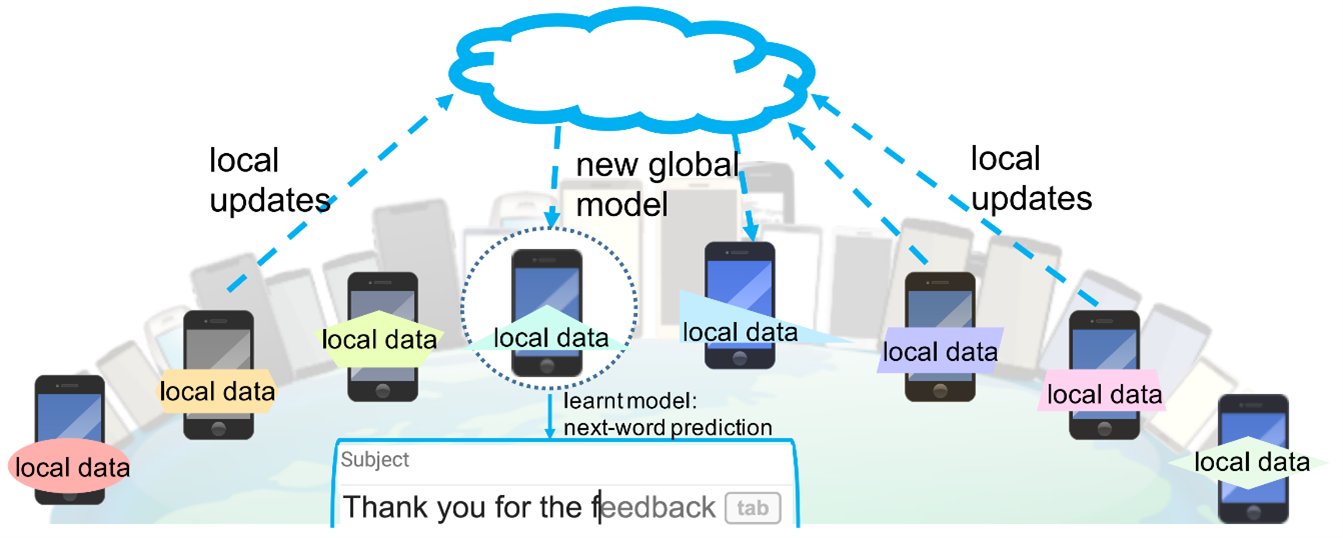
\includegraphics[scale=1]{images/chap1/gboard.png}%
	\caption{%
استفاده از یادگیری فدرال برای پیش‌بینی کلمه بعدی در
\lr{Gboard}
		\cite{li2020federated}%
		.
	}
	\label{gboard}
	\centering
\end{figure}



\section{کاربرد یادگیری فدرال}
سامانه‌های متمرکز سنتی که تنها مسئول جمع‌آوری، پایش و کنترل شرایط به صورت محلی بودند، اکنون جای خود را به دستگاه‌های هوشمندی داده‌اند که قابلیت پردازش و برنامه‌ریزی داده‌ها را در سطح سیار و سیستمی دارند. علاوه بر این، گسترش ارتباطات مبتنی بر اینترنت، امکان انتقال و تبادل داده‌ها بین سیستم‌های مختلف را فراهم کرده است. این تحولات منجر به کاهش نیاز به تصمیم‌گیری متمرکز و توسعه سیستم‌های کنترل و پایش پیشرفته شده است. این ویژگی‌ها، همراه با حجم روزافزون داده‌ها، یادگیری فدرال را به یکی از بهترین روش‌ها برای توسعه سیستم‌های هوشمند تبدیل کرده است
\cite{mahtab2022algorithm}.
در ادامه، سه نمونه از کاربردهای یادگیری فدرال شرح داده خواهد شد.


\subsection{یادگیری فدرال در شهر هوشمند}
در یک شهر هوشمند%
\LTRfootnote{Smart City}%
، اطلاعات جمع‌آوری شده از حسگرهای مختلف مانند داده‌های ترافیک، مصرف انرژی، پسماند شهری و رویدادهای امنیتی، ارزش بالایی دارند و به عنوان منبعی کلیدی برای بهبود عملکرد شهر هوشمند و ارتقای کیفیت زندگی شهروندان محسوب می‌شوند. اما در کنار این مزایا، حفظ حریم شخصی و امنیت اطلاعات شهروندان نیز از اهمیت بالایی برخوردار است. در اینجا یادگیری فدرال به عنوان یک رویکرد نوین که مبتنی بر حفظ حریم شخصی است، به کار گرفته می‌شود.

در یک شهر هوشمند، سازمان‌های مختلف هر کدام اطلاعات خاص خود را دارند، اما این اطلاعات به طور متقابل بر یکدیگر تأثیر می‌گذارند و می‌توانند در مدیریت بهینه شهر نقش مهمی ایفا کنند. یادگیری فدرال با حفظ حریم شخصی کاربران، این امکان را فراهم می‌کند که سازمان‌ها بدون نیاز به اشتراک‌گذاری داده‌های حساس خود با یکدیگر، از داده‌های موجود بهره‌برداری کنند و مدل‌های هوش مصنوعی و الگوریتم‌های بهبود عملکرد شهر هوشمند را توسعه دهند. به عنوان مثال، با استفاده از یادگیری فدرال می‌توان بهبود مدیریت ترافیک، بهینه‌سازی مصرف انرژی، کاهش آلودگی هوا و افزایش امنیت شهری را تحقق بخشید، در حالی که حریم شخصی شهروندان به بهترین نحو ممکن حفظ می‌شود.


\subsection{یادگیری فدرال در بیمارستان}
در یک بیمارستان، اطلاعات پزشکی به شدت حساس و مهم هستند و باید به صورت محرمانه نگهداری شوند. با این حال، بهره‌برداری از این داده‌ها برای ارتقاء خدمات بهداشتی و درمانی بسیار ارزشمند است. در این شرایط، یادگیری فدرال می‌تواند نقش مهمی ایفا کند. با استفاده از روش‌های یادگیری فدرال، بیمارستان‌ها می‌توانند از داده‌های پزشکی بیماران خود برای توسعه مدل‌هایی استفاده کنند که به بهبود خدمات، ارتقاء روش‌های تشخیص و درمان بیماری‌ها و افزایش بهره‌وری پزشکان کمک می‌کنند، بدون اینکه نیاز باشد این داده‌ها به طور مستقیم به یک مرکز جمع‌آوری اطلاعات ارسال شوند.

به عنوان نمونه، یادگیری فدرال این امکان را فراهم می‌کند که مدل‌های هوش مصنوعی روی داده‌های محلی بیماران در هر بیمارستان آموزش ببینند و بیماری‌ها را شناسایی و تشخیص دهند. این فرایند به بهبود درمان‌ها کمک می‌کند، بدون اینکه اطلاعات حساس بیماران به بیرون درز کند و امنیت آن‌ها حفظ می‌شود. در شکل
\ref{hospital}
یک نمونه استفاده از یادگیری فدرال در بیمارستان‌ها به نمایش در آمده است.


\begin{figure}[t]
	\centering
	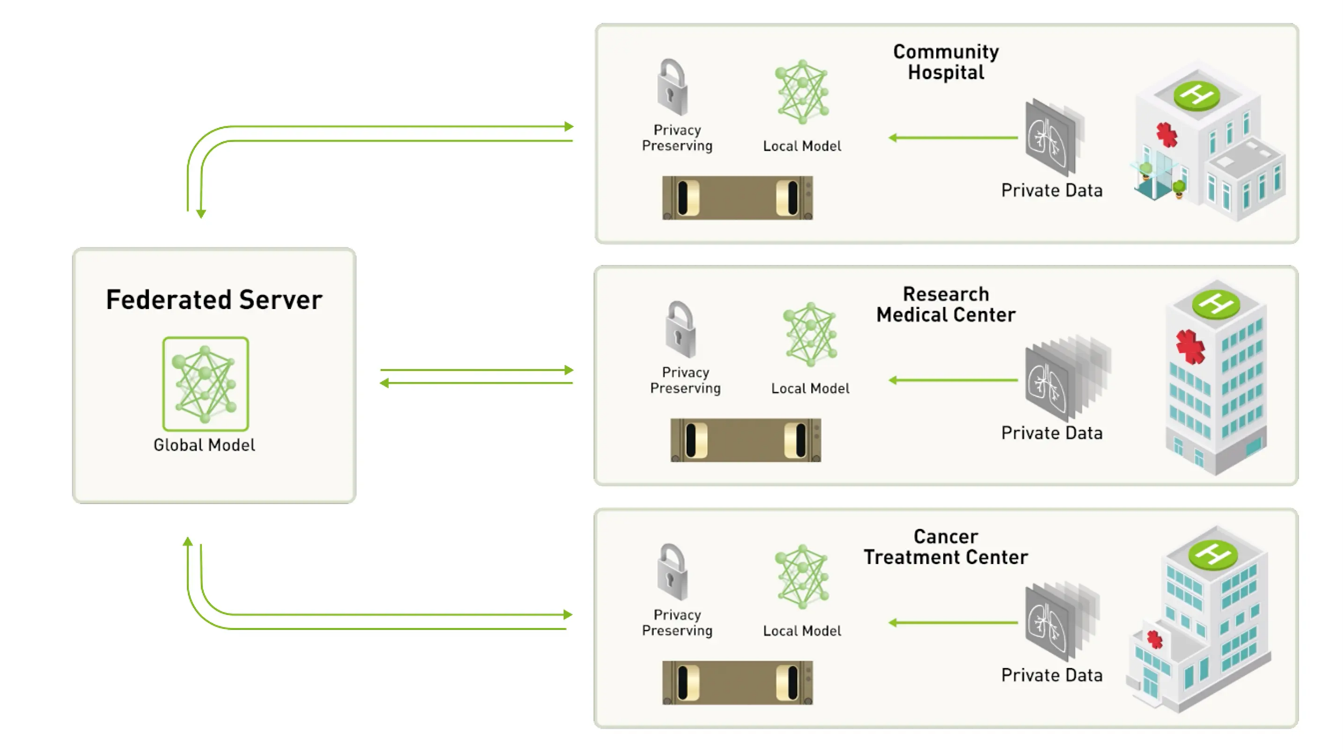
\includegraphics[scale=1]{images/chap1/hospital.png}%
	\caption{%
		یادگیری فدرال در بیمارستان
		\cite{rieke2019what}%
		.
	}
	\label{hospital}
	\centering
\end{figure}



\subsection{یادگیری فدرال در فروشگاه برنامه‌های کاربردی تلفن‌همراه}

یک فروشگاه مجازی برنامه‌های کاربردی%
\LTRfootnote{App Store}
تلفن‌همراه را در نظر بگیرید که به کاربران امکان دریافت و نصب برنامه‌های مختلف را می‌دهد. این فروشگاه می‌خواهد با استفاده از داده‌های کاربران خود، الگوریتمی را توسعه دهد که بتواند به طور دقیق‌تری برنامه‌های مورد علاقه کاربران را به آن‌ها پیشنهاد دهد. اگر این فروشگاه از روش‌های متمرکز استفاده کند، باید داده‌های حساس و شخصی کاربران را جمع‌آوری و تحلیل کند، که این موضوع می‌تواند نگرانی‌های جدی در مورد حریم خصوصی کاربران ایجاد کند و غیر عملی باشد.

در حالی که با استفاده از یادگیری فدرال، این فروشگاه می‌تواند الگوریتم خود را بر روی داده‌های محلی هر کاربر اجرا کند. به این ترتیب، هیچ داده حساسی به یک مرکز جمع‌آوری داده‌ها ارسال نمی‌شود و حریم خصوصی کاربران حفظ می‌گردد. به عنوان مثال، اگر یک کاربر به برنامه‌های موسیقی علاقه‌مند باشد، الگوریتم محلی در تلفن هوشمند او می‌تواند این الگو را شناسایی کند و پیشنهادات مربوط به برنامه‌های موسیقی را ارائه دهد، بدون اینکه نیاز به ارسال داده‌های شخصی و حساس او به سرور فروشگاه باشد.


\section{دید کلی از روند موضوع و بیان هدف پژوهش}
تکمیل این بخش پس از رسیدن به ساختار کلی پایان‌نامه (چون ممکنه در ادامه تغییر کنه)

چند جلمه کلیدی:

به دلیل پراکندگی همگرایی به کندی صورت می‌گیرد

روش جابجایی وزن‌ها بین کاربران نهایی در طول فرایند

چرا جابجایی تصادفی، جابجایی هوشمند بر اساس میزان شباهت

\section{مروی بر روند ارائه مطالب پایان‌نامه}
تست

